\documentclass[border=8pt, multi, tikz]{standalone} 
\usepackage{import}
\usepackage{tikz}
\subimport{layers/}{init}
\usetikzlibrary{positioning}
\usetikzlibrary{3d} %for including external image 

\def\ConvColor{rgb:yellow,5;red,2.5;white,5}
\def\ConvReluColor{rgb:yellow,5;red,5;white,5}
\def\PoolColor{rgb:orange,1;black,0.3}
\def\UnpoolColor{rgb:blue,2;green,1;black,0.3}
\def\FcColor{rgb:blue,5;red,2.5;white,5}
\def\FcReluColor{rgb:blue,5;red,5;white,4}
\def\SoftmaxColor{rgb:magenta,5;black,7}   
\def\SumColor{rgb:blue,5;green,15}

\def\DcnvColor{rgb:blue,1;orange,2;white,2.5}
\def\DenseBlockColor{rgb:orange,3;black,0.8}
\def\DenseTransferColor{rgb:orange,2;red,3;black,1.2}
\def\TransitionColor{rgb:blue,5;green,2.5;white,2.5}
\def\ClassierColor{rgb:blue,5;green,2.5;white,2.5}
\def\ConcatColor{rgb:yellow,5;red,2;black,2}

\newcommand{\copymidarrow}{\tikz \draw[-Stealth,line width=0.8mm,draw={rgb:blue,4;red,1;green,1;black,3}] (-0.3,0) -- ++(0.3,0);}

\begin{document}
\begin{tikzpicture}
\tikzstyle{connection}=[ultra thick,every node/.style={sloped,allow upside down},draw=\edgecolor,opacity=0.7]
\tikzstyle{copyconnection}=[ultra thick,every node/.style={sloped,allow upside down},draw={rgb:blue,4;red,1;green,1;black,3},opacity=0.7]

% 导入rgb 图片 和亮度图片
\node[canvas is yz plane at x=0] (RGB) at (-3,0,0) {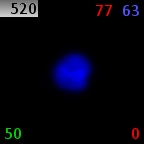
\includegraphics[width=8cm,height=8cm,angle=270]{1.jpg}};
\node[canvas is yz plane at x=0] (Light) at (-3,-15,0) {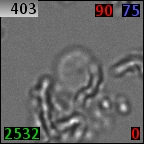
\includegraphics[width=8cm,height=8cm,angle=270]{2.jpg}};

% 导入第一层变换层
\pic[shift={(0,0,0)}] at (0,0,0) {Box={name=RGBConvlution,caption=R Cov,fill=\DenseTransferColor,opacity=0.5,height=30,width=3,depth=30}};
\pic[shift={(0,-15,0)}] at (0,0,0) {Box={name=LightConvlution,caption=L Cov,fill=\DenseTransferColor,opacity=0.5,height=30,width=3,depth=30}};


% RGB block1 内部 6 层
\pic[shift={(4,0,0)}] at (RGBConvlution-east) {Box={name=block1rd1,xlabel={{"","dummy"}},fill=\DcnvColor,opacity=0.7,height=40,width=2,depth=40}};
\pic[shift={(.15,0,0)}] at (block1rd1-east) {Box={name=block1rd2,xlabel={{"","dummy"}},fill=\DcnvColor,opacity=0.7,height=40,width=2,depth=40}};
\pic[shift={(.15,0,0)}] at (block1rd2-east) {Box={name=block1rd3,xlabel={{"","dummy"}},fill=\DcnvColor,opacity=0.7,height=40,width=2,depth=40}};
\pic[shift={(.15,0,0)}] at (block1rd3-east) {Box={name=block1rd4,xlabel={{"","dummy"}},fill=\DcnvColor,opacity=0.7,height=40,width=2,depth=40}};
\pic[shift={(.15,0,0)}] at (block1rd4-east) {Box={name=block1rd5,xlabel={{"","dummy"}},fill=\DcnvColor,opacity=0.7,height=40,width=2,depth=40}};
\pic[shift={(.15,0,0)}] at (block1rd5-east) {Box={name=block1rd6,xlabel={{"","dummy"}},fill=,opacity=0.01,height=40,width=2,depth=40}};
% light block1 内部 6 层
\pic[shift={(4,0,0)}] at (LightConvlution-east) {Box={name=block1ld1,xlabel={{"","dummy"}},fill=\DcnvColor,opacity=0.7,height=40,width=2,depth=40}};
\pic[shift={(.15,0,0)}] at (block1ld1-east) {Box={name=block1ld2,xlabel={{"","dummy"}},fill=\DcnvColor,opacity=0.7,height=40,width=2,depth=40}};
\pic[shift={(.15,0,0)}] at (block1ld2-east) {Box={name=block1ld3,xlabel={{"","dummy"}},fill=\DcnvColor,opacity=0.7,height=40,width=2,depth=40}};
\pic[shift={(.15,0,0)}] at (block1ld3-east) {Box={name=block1ld4,xlabel={{"","dummy"}},fill=\DcnvColor,opacity=0.7,height=40,width=2,depth=40}};
\pic[shift={(.15,0,0)}] at (block1ld4-east) {Box={name=block1ld5,xlabel={{"","dummy"}},fill=\DcnvColor,opacity=0.7,height=40,width=2,depth=40}};
\pic[shift={(.15,0,0)}] at (block1ld5-east) {Box={name=block1ld6,xlabel={{"","dummy"}},fill=,opacity=0.01,height=40,width=2,depth=40}};
% dense block1 外部矩形块
\pic[shift={(-0.2,0,0)}] at (4.5,0,0) {Box={name=RGBblock1,caption=RGB Dense Block 1,xlabel={{"","dummy"}},fill=\DenseBlockColor,opacity=0.4,height=40,width={19},depth=40}};
\pic[shift={(-0.2,0,0)}] at (4.5,-15,0) {Box={name=Lightblock1,caption=Light Dense Block 1,xlabel={{"","dummy"}},fill=\DenseBlockColor,opacity=0.4,height=40,width={19},depth=40}};

% RGB block2 内部 12 层
\pic[shift={(4,0,0)}] at (RGBblock1-east) {Box={name=block2rd1,xlabel={{"","dummy"}},fill=\DcnvColor,opacity=0.7,height=40,width=2,depth=40}};
\pic[shift={(.15,0,0)}] at (block2rd1-east) {Box={name=block2rd2,xlabel={{"","dummy"}},fill=\DcnvColor,opacity=0.7,height=40,width=2,depth=40}};
\pic[shift={(.15,0,0)}] at (block2rd2-east) {Box={name=block2rd3,xlabel={{"","dummy"}},fill=\DcnvColor,opacity=0.7,height=40,width=2,depth=40}};
\pic[shift={(.15,0,0)}] at (block2rd3-east) {Box={name=block2rd4,xlabel={{"","dummy"}},fill=\DcnvColor,opacity=0.7,height=40,width=2,depth=40}};
\pic[shift={(.15,0,0)}] at (block2rd4-east) {Box={name=block2rd5,xlabel={{"","dummy"}},fill=\DcnvColor,opacity=0.7,height=40,width=2,depth=40}};
\pic[shift={(.15,0,0)}] at (block2rd5-east) {Box={name=block2rd6,xlabel={{"","dummy"}},fill=\DcnvColor,opacity=0.7,height=40,width=2,depth=40}};
\pic[shift={(.15,0,0)}] at (block2rd6-east) {Box={name=block2rd7,xlabel={{"","dummy"}},fill=\DcnvColor,opacity=0.7,height=40,width=2,depth=40}};
\pic[shift={(.15,0,0)}] at (block2rd7-east) {Box={name=block2rd8,xlabel={{"","dummy"}},fill=\DcnvColor,opacity=0.7,height=40,width=2,depth=40}};
\pic[shift={(.15,0,0)}] at (block2rd8-east) {Box={name=block2rd9,xlabel={{"","dummy"}},fill=\DcnvColor,opacity=0.7,height=40,width=2,depth=40}};
\pic[shift={(.15,0,0)}] at (block2rd9-east) {Box={name=block2rd10,xlabel={{"","dummy"}},fill=\DcnvColor,opacity=0.7,height=40,width=2,depth=40}};
\pic[shift={(.15,0,0)}] at (block2rd10-east) {Box={name=block2rd11,xlabel={{"","dummy"}},fill=\DcnvColor,opacity=0.7,height=40,width=2,depth=40}};
\pic[shift={(.15,0,0)}] at (block2rd11-east) {Box={name=block2rd12,xlabel={{"","dummy"}},fill=,opacity=0.01,height=40,width=2,depth=40}};
% light block2 内部 12 层
\pic[shift={(4,0,0)}] at (Lightblock1-east) {Box={name=block2ld1,xlabel={{"","dummy"}},fill=\DcnvColor,opacity=0.7,height=40,width=2,depth=40}};
\pic[shift={(.15,0,0)}] at (block2ld1-east) {Box={name=block2ld2,xlabel={{"","dummy"}},fill=\DcnvColor,opacity=0.7,height=40,width=2,depth=40}};
\pic[shift={(.15,0,0)}] at (block2ld2-east) {Box={name=block2ld3,xlabel={{"","dummy"}},fill=\DcnvColor,opacity=0.7,height=40,width=2,depth=40}};
\pic[shift={(.15,0,0)}] at (block2ld3-east) {Box={name=block2ld4,xlabel={{"","dummy"}},fill=\DcnvColor,opacity=0.7,height=40,width=2,depth=40}};
\pic[shift={(.15,0,0)}] at (block2ld4-east) {Box={name=block2ld5,xlabel={{"","dummy"}},fill=\DcnvColor,opacity=0.7,height=40,width=2,depth=40}};
\pic[shift={(.15,0,0)}] at (block2ld5-east) {Box={name=block2ld6,xlabel={{"","dummy"}},fill=\DcnvColor,opacity=0.7,height=40,width=2,depth=40}};
\pic[shift={(.15,0,0)}] at (block2ld6-east) {Box={name=block2ld7,xlabel={{"","dummy"}},fill=\DcnvColor,opacity=0.7,height=40,width=2,depth=40}};
\pic[shift={(.15,0,0)}] at (block2ld7-east) {Box={name=block2ld8,xlabel={{"","dummy"}},fill=\DcnvColor,opacity=0.7,height=40,width=2,depth=40}};
\pic[shift={(.15,0,0)}] at (block2ld8-east) {Box={name=block2ld9,xlabel={{"","dummy"}},fill=\DcnvColor,opacity=0.7,height=40,width=2,depth=40}};
\pic[shift={(.15,0,0)}] at (block2ld9-east) {Box={name=block2ld10,xlabel={{"","dummy"}},fill=\DcnvColor,opacity=0.7,height=40,width=2,depth=40}};
\pic[shift={(.15,0,0)}] at (block2ld10-east) {Box={name=block2ld11,xlabel={{"","dummy"}},fill=\DcnvColor,opacity=0.7,height=40,width=2,depth=40}};
\pic[shift={(.15,0,0)}] at (block2ld11-east) {Box={name=block2ld12,xlabel={{"","dummy"}},fill=,opacity=0.01,height=40,width=2,depth=40}};
% dense block2 外部矩形块
\pic[shift={(3.7,0,0)}] at (RGBblock1-east) {Box={name=RGBblock2,caption=RGB Dense Block 2,xlabel={{"","dummy"}},fill=\DenseBlockColor,opacity=0.4,height=40,width={36},depth=40}};
\pic[shift={(3.7,0,0)}] at (Lightblock1-east) {Box={name=Lightblock2,caption=Light Dense Block 2,xlabel={{"","dummy"}},fill=\DenseBlockColor,opacity=0.4,height=40,width={36},depth=40}};

% RGB block3 内部 12 层
\pic[shift={(4,0,0)}] at (RGBblock2-east) {Box={name=block3rd1,xlabel={{"","dummy"}},fill=\DcnvColor,opacity=0.7,height=40,width=2,depth=40}};
\pic[shift={(.15,0,0)}] at (block3rd1-east) {Box={name=block3rd2,xlabel={{"","dummy"}},fill=\DcnvColor,opacity=0.7,height=40,width=2,depth=40}};
\pic[shift={(.15,0,0)}] at (block3rd2-east) {Box={name=block3rd3,xlabel={{"","dummy"}},fill=\DcnvColor,opacity=0.7,height=40,width=2,depth=40}};
\pic[shift={(.15,0,0)}] at (block3rd3-east) {Box={name=block3rd4,xlabel={{"","dummy"}},fill=,opacity=0.01,height=40,width=2,depth=40}};
% light block3 内部 12 层
\pic[shift={(4,0,0)}] at (Lightblock2-east) {Box={name=block3ld1,xlabel={{"","dummy"}},fill=\DcnvColor,opacity=0.7,height=40,width=2,depth=40}};
\pic[shift={(.15,0,0)}] at (block3ld1-east) {Box={name=block3ld2,xlabel={{"","dummy"}},fill=\DcnvColor,opacity=0.7,height=40,width=2,depth=40}};
\pic[shift={(.15,0,0)}] at (block3ld2-east) {Box={name=block3ld3,xlabel={{"","dummy"}},fill=\DcnvColor,opacity=0.7,height=40,width=2,depth=40}};
\pic[shift={(.15,0,0)}] at (block3ld3-east) {Box={name=block3ld4,xlabel={{"","dummy"}},fill=,opacity=0.01,height=40,width=2,depth=40}};
% dense block3 外部矩形块
\pic[shift={(3.7,0,0)}] at (RGBblock2-east) {Box={name=RGBblock3,caption=RGB Dense Block 3,xlabel={{"","dummy"}},fill=\DenseBlockColor,opacity=0.4,height=40,width={14},depth=40}};
\pic[shift={(3.7,0,0)}] at (Lightblock2-east) {Box={name=Lightblock3,caption=Light Dense Block 3,xlabel={{"","dummy"}},fill=\DenseBlockColor,opacity=0.4,height=40,width={14},depth=40}};

% transition
\pic[shift={(4.5,0,0)}] at (RGBblock3-east) {Box={name=Rtransition,caption=RGB Trainsition Layer,xlabel={{"","dummy"}},fill=\TransitionColor,opacity=0.4,height=20,width={14},depth=60}};
\pic[shift={(4.5,0,0)}] at (Lightblock3-east) {Box={name=Ltransition,caption=Light Trainsition Layer,xlabel={{"","dummy"}},fill=\TransitionColor,opacity=0.4,height=20,width={14},depth=60}};

%concat
\pic[shift={(0,7,0)}] at (Ltransition-anchor) {Ball={name=cat4,fill=cyan!70,radius=2.5,logo=$||$}};
\pic[shift={(6,3,0)}] at (cat4-east) {Box={name=Concat,caption=Concat Out,xlabel={{"","dummy"}},fill=\ConcatColor,opacity=0.4,height=20,width={14},depth=60}};
% classifier
%\pic[shift={(3.7,0,0)}] at (cat4) {Box={name=Classifer,caption=concat,fill=\DenseBlockColor,opacity=0.4,height=40,width={14},depth=40}};

%链接
\draw [connection]  (RGBConvlution-east) -- node{\midarrow} (RGBblock1-west);
\draw [connection]  (LightConvlution-east) -- node{\midarrow}  (Lightblock1-west);

\draw [connection]  (RGBblock1-east) -- node{\midarrow} (RGBblock2-west);
\draw [connection]  (Lightblock1-east) -- node{\midarrow} (Lightblock2-west);

\draw [connection]  (RGBblock2-east) -- node{\midarrow} (RGBblock3-west);
\draw [connection]  (Lightblock2-east) -- node{\midarrow} (Lightblock3-west);

\draw [connection]  (RGBblock3-east) -- node{\midarrow} (Rtransition-west);
\draw [connection]  (Lightblock3-east) -- node{\midarrow} (Ltransition-west);

\draw [connection]  (Ltransition-north) -- node{\midarrow} (cat4-south);
\draw [connection]  (Rtransition-south) -- node{\midarrow} (cat4-north);


\draw[densely dashed]
(Rtransition-nearnortheast) -- (Concat-nearnorthwest)


(Rtransition-farnortheast)  -- (Concat-farnorthwest)


(Ltransition-nearsoutheast) -- (Concat-nearsouthwest)
(Ltransition-farsoutheast)  -- (Concat-farsouthwest)

;
\end{tikzpicture}
\end{document}




































